\subsection{Bill of Materials}
The bill of materials for a single Aether node can be found in Table \ref{tab:bom}.

\begin{table}
\centering\scriptsize
\caption{The bill of materials for a single Aether node.}
\begin{tabular}{|l|l|l|l|l|}
\hline
Part Name & Part Value & Quantity & Unit Cost & Cost \\ 
\hline\hline
Thermristor & 10k & 1 & \$5.00 & \$5.00 \\\hline

\end{tabular}
\label{tab:bom}
\end{table}




\begin{figure}
    \centering
    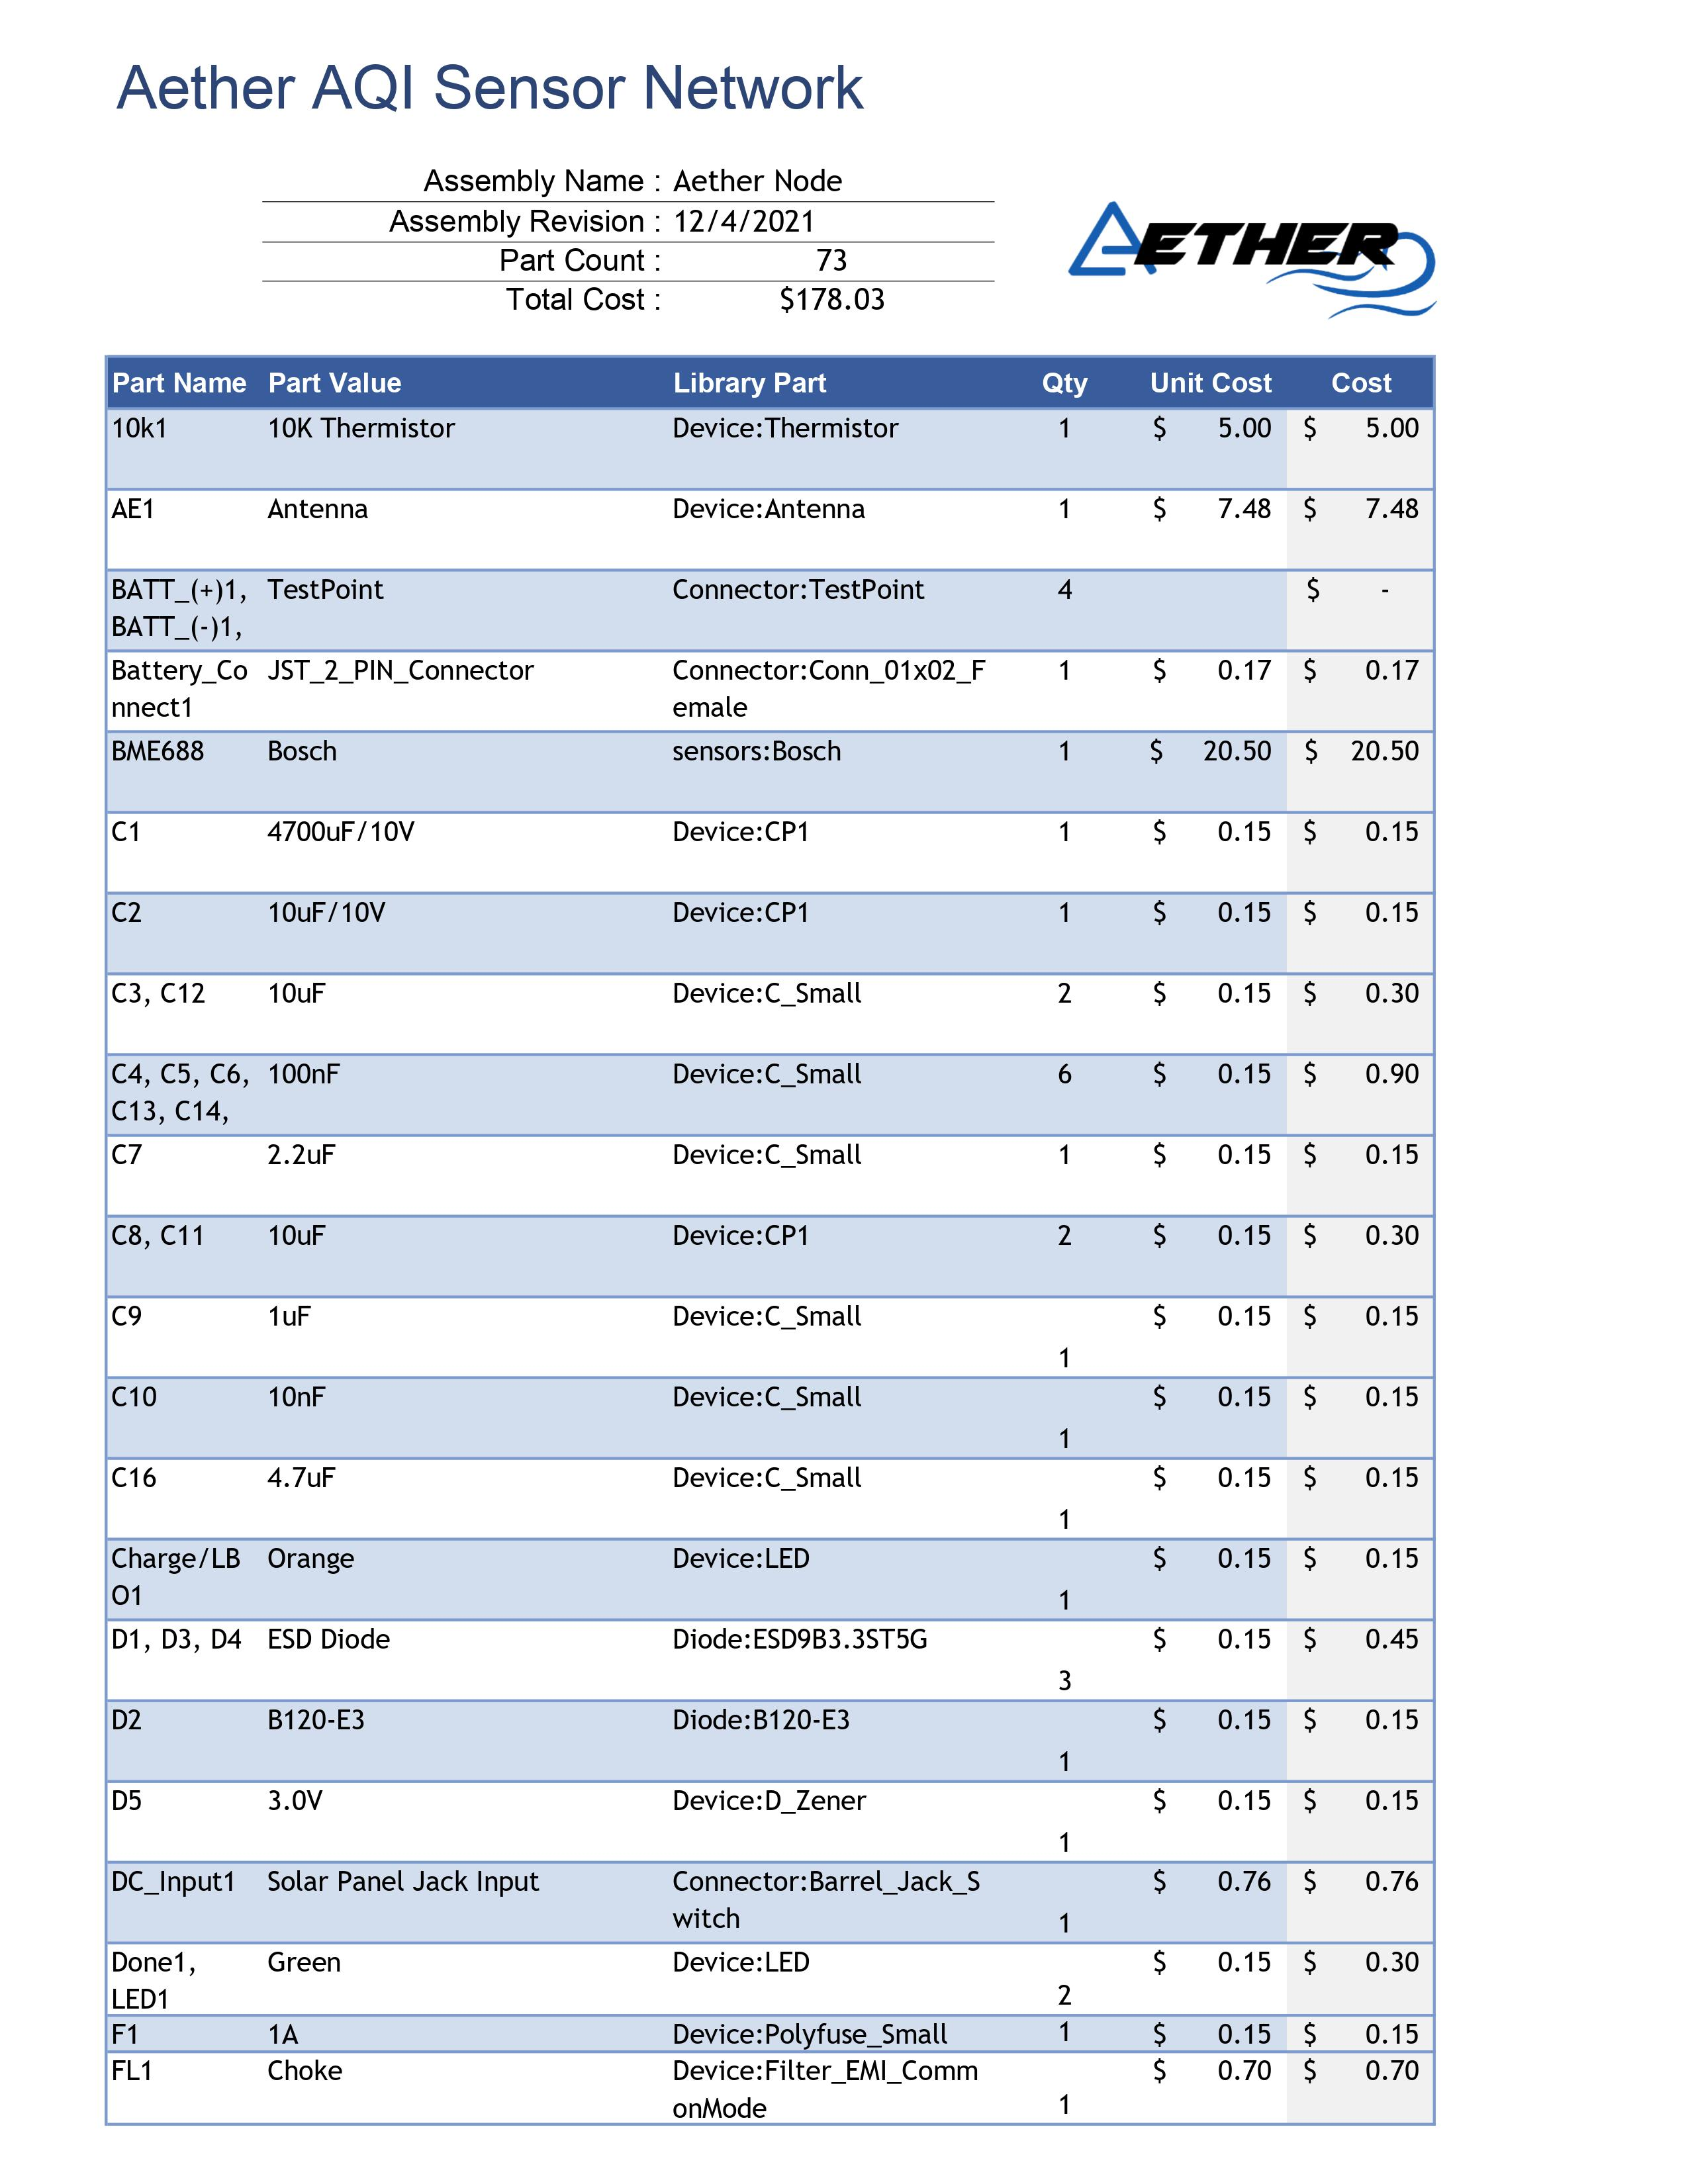
\includegraphics[width=6in]{figures/BOM_1.jpg}
    \label{fig:BOM_1} 
\end{figure}
\begin{figure}
    \centering
    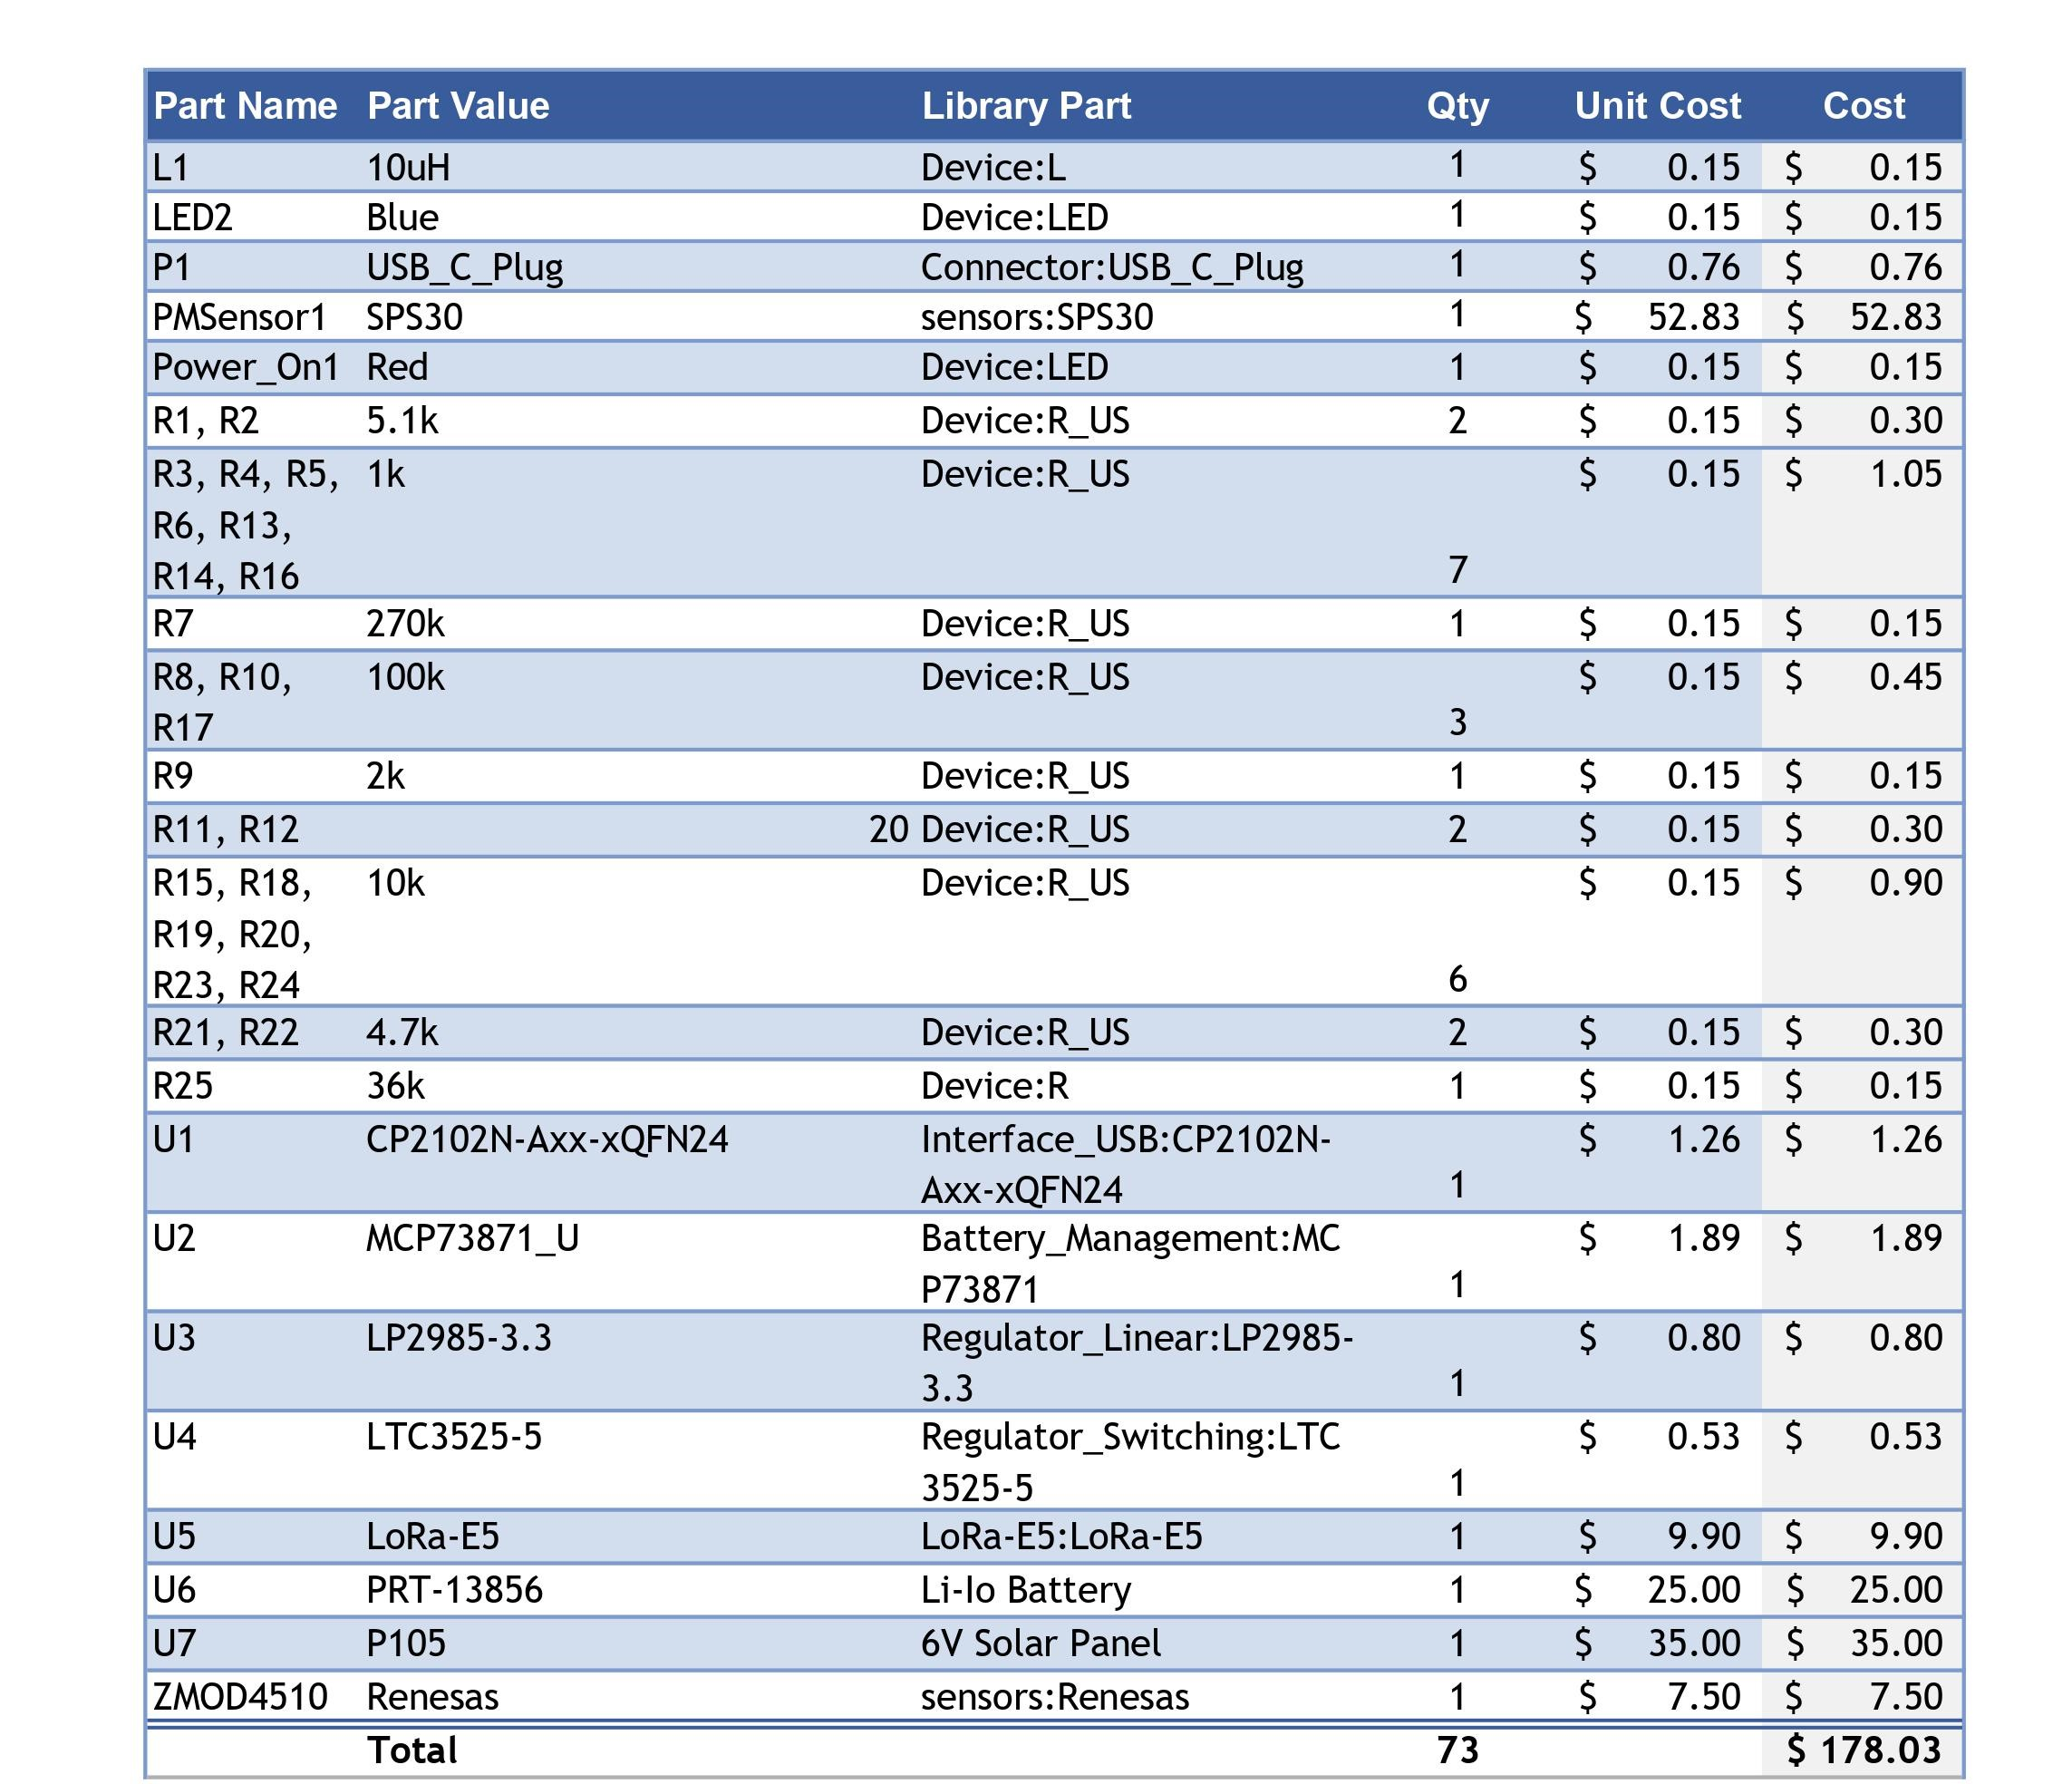
\includegraphics[width=6in]{figures/BOM_2.jpg}
    \caption{Aether Node BOMl}
    \label{fig:BOM_2} 
\end{figure}